
\begin{section}{Teachers}

    This section provides an overview of all functionality a teacher is offered
    on our application.

    \begin{subsection}{Inheritance}

        The teacher can do many things also available for other users. These are
        listed below. More explanation can be found with the respective users
        they share these functionality with.

        \begin{subsubsection}{Independent}

            \begin{itemize}
                \item Change password           (\ref{indep-pass});
                \item Change email address     (\ref{indep-email});
                \item Change preferred language (\ref{indep-lang});
                \item Log out                   (\ref{indep-logout}).
            \end{itemize}

        \end{subsubsection}

    \end{subsection}

    \begin{subsection}{General functionality}
	The teacher will use a lot of specifications given by the organizer (like managing personal information, pupils, classes etc.). In general a teacher can do the following actions.\\

    \begin{subsubsection}{Change personal information}
	When the teacher logs in he will come to a personal web page. On this page, at first, he can see
	\begin{itemize}
		\item Personal information
		\item School's information
		\item Login information
	\end{itemize}	
	Beneath the personal information form there is placed an edit button which provides an edit functionality.
	The School's information form shows information about the schools to which the teacher is linked. Also there is some general
	information for each school like the website, name, email address and telephone number.\\
	\\
	Under the login information part there is an 'Edit password' button. 
	This button brings the teacher to a webpage where he can fill in his current password and new password. 
	After clicking 'Change', the current password is being checked before the changes take place.
	\end{subsubsection}
	\begin{subsubsection}{Register pupil/class}
	Information of this part can be found under section \nameref{sec:organizer}.\\
	Although it is import to mention that the registration and assigning is done by uploading a CSV file to the server, it's also important to note that there is only one problem with the use of a CSV file. When a pupil is registrated and he	was already been registrated before (to another class), this pupil must be merged to the current ID in order to avoid
	redundancy.\\
	So a check for every pupil must be done while uploading a CSV. \\
	When it comes to registering a class, the teacher goes to a special web page called the classgroup web page. On this page
	the teacher can add a classgroup to an existing list of available classgroups within the application. There is a button
	'Add classgroup' which brings the teacher to a page where he can see a list with all the registrated pupils. Next to every
	pupil there is a green '+' button and '-' button (if the pupil is already in the classgroup list). These add/remove buttons
	are used in order to add/remove a pupil from the current classgroup which is being registrated.\\
	\begin{figure}[!h]
			  \centering
				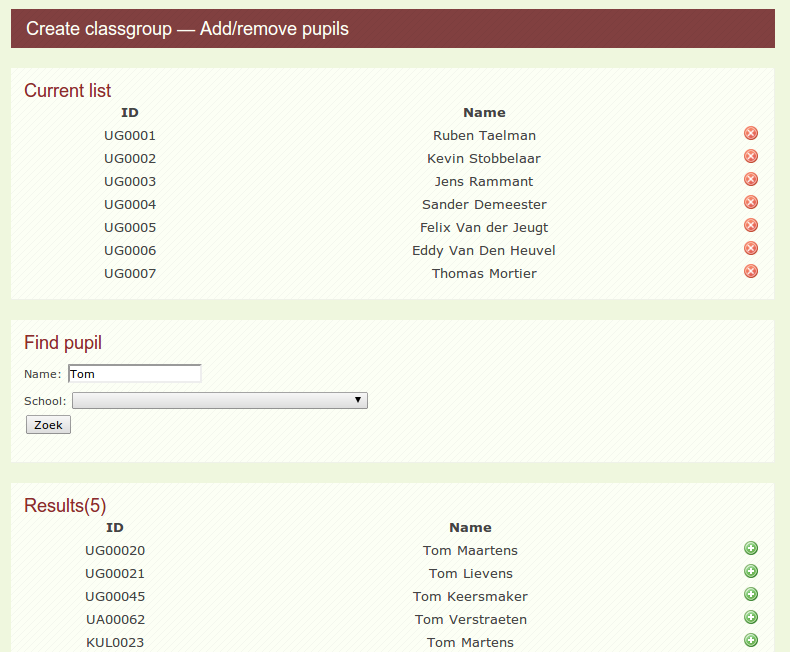
\includegraphics[width=1\textwidth]{img/add_remove_pupil_classgroup.png}
			  \caption{How creating a classgroup is done}
			  \label{create_classgroup}
			\end{figure}
	After all the pupils are in the list, the teacher can click 'Add classgroup' which adds this group to the existing list
	of classgroups. 
	\end{subsubsection}
	\begin{subsubsection}{Open and close (local) competition}
	Also this is very similar as in the section about organizers. The teacher will use the organizer's competition page.
	On this page the teacher can simply add classes which he has registered as described in section Register pupil/ class.
	A class must be added in order to participate in the official Bebras competition. After adding a class the teacher can
	close the competition.\\
	\end{subsubsection}
	\begin{subsubsection}{Get restricted question set}
	Since the teacher can open/close a competition he must also have access to the restricted question sets. This is done by going
	to the 'competition management' as described in the section \nameref{sec:organizer}. On this page he can view all sets of questions.
	\end{subsubsection}
	\begin{subsubsection}{Get marks}
	After the competition has closed, the teacher can view the marks of the pupils which are saved on the server.\\
	This could be done by opening a competition and using the 'Get Marks' button which opens the specific file.
	\end{subsubsection}
	\begin{subsubsection}{Get state of pupil}
	As described in the SRS, the teacher can monitor his pupils while joining a competition. This is done on the overview screen of 		the current running competition. On this page a 'View stats' button is available which displays a live table 
	(i.e. a table which is dynamically updated during the running competition). This table shows information like if they are logged 		in, if they had already pressed the finish button or the time left. 
	\end{subsubsection}
	\begin{subsubsection}{Grant pupil minutes}
	When the teacher goes to the running competition page he can see next to the stats (of the running competition) also a table with 		all the participants of that competition. For each pupil he can see the 'time left' (sort of label) in the competition. It is also 		possible for the teacher to add/remove some minutes of a pupil. This is done by clicking on an arrow button which increase/decrease 		the 'time left' value.
    \end{subsubsection}
    \end{subsection}

\end{section}
